% 数字图像处理课程实验报告。使用 XeLaTeX / latexmk 编译。
\documentclass[UTF8,a4paper,zihao=5,fontset=fandol,twoside]{ctexart}
\usepackage[asymmetric,left=18.4mm,right=19.6mm,top=38.8mm,bottom=23.2mm,headheight=16pt,headsep=23.4pt]{geometry}
\usepackage{graphicx,amsmath,amssymb,booktabs,tabularx,array}
\usepackage{caption,fancyhdr,float,fvextra,needspace,placeins}
\usepackage{gbt7714}
\usepackage[hidelinks,unicode]{hyperref}

\setmonofont{DejaVu Sans Mono}
\setCJKfamilyfont{reportcode}{FandolFang-Regular.otf}
\captionsetup{font=normalsize,labelfont=bf,labelsep=quad,skip=6pt}
\captionsetup[figure]{name=Fig.}
\captionsetup[table]{name=Table}
\ctexset{section={format=\large\heiti\bfseries},subsection={format=\normalsize\songti\bfseries}}
\graphicspath{{figures/}{../../task4/}{../../task2/param/param_fixed/}{../../task3/output/bicubic/RealBlur/}}
\setlength{\parindent}{2em}
\setlength{\emergencystretch}{1em}
\setlength{\textfloatsep}{12pt plus 3pt minus 2pt}
\setlength{\intextsep}{11pt plus 3pt minus 2pt}
\raggedbottom
\linespread{1.409}

\newcommand{\ReportTitle}{退化图像的传统频域复原与对照实验}
\newcommand{\ReportMonth}{2026 年 11 月}
\newcommand{\ReportAuthors}{李建辉，苏威贤，王妍，李定一}

% 按课程参考稿设置奇偶页页眉，页码位于外侧。
\pagestyle{fancy}
\fancyhf{}
\fancyhead[LE]{\zihao{-5}\hspace*{4.3mm}\thepage}
\fancyhead[CE]{\zihao{-5}\hspace*{3.6mm}数字图像处理}
\fancyhead[RE]{\zihao{-5}\ReportMonth\hspace*{3.1mm}}
\fancyhead[LO]{\zihao{-5}\hbox to \headwidth{%
  \hspace*{3.25mm}\ReportAuthors\hfil\ReportTitle\hfil\thepage\hspace*{3.25mm}}}
\renewcommand{\headrulewidth}{0.5pt}
\hypersetup{pdftitle={\ReportTitle},pdfauthor={\ReportAuthors}}
\renewcommand{\bibsection}{\section*{参考文献}}

\begin{document}

\thispagestyle{empty}
\noindent{\zihao{-5}\ReportAuthors\hfill DIP \& \ReportTitle\hfill \ReportMonth}\par
\noindent\rule[0.25\baselineskip]{\textwidth}{1pt}
\begin{center}
\vspace{9mm}
{\zihao{2}\heiti \ReportTitle\par}
\vspace{3mm}
{\zihao{4}\fangsong 李建辉\quad 苏威贤\quad 王妍\quad 李定一\par}
\vspace{2mm}
{\large\bfseries Frequency-Domain Restoration of Degraded Images\par}
\end{center}

\begingroup
\zihao{5}
\setlength{\baselineskip}{16pt}
\noindent{\heiti 摘\quad 要}\quad
在已知退化模型与未知真实运动核两种条件下，对比逆滤波、维纳滤波和约束最小二乘复原（CLS）。
用一张 DIV2K 清晰图生成两个高斯核尺寸与三种边界方式的六组带噪退化图。
对一组 RealBlur-J 实拍图使用四种假设高斯核，并设置双三次插值和非局部均值（NLM）对照。
DIV2K 的 \(15\times15\) 反射延拓组中，维纳滤波将 PSNR 从 24.8606 dB 提高到 26.8605 dB，
SSIM 从 0.64326 提高到 0.77884。两种核尺寸的周期延拓组均从循环卷积模型的边界一致性中受益。
RealBlur-J 的高斯猜核在所测主实验参数下低于原始退化图，插值和 NLM 的指标仅小幅变化。
选做实验中，由 Radon 变换估计的直线运动核结合维纳滤波达到 20.3334 dB 和 0.60804，
但文字拖尾仍有残留。实验展示了去卷积增益对核、边界与正则化设置的依赖。\par
\vspace{5mm}
\noindent{\heiti 关键词}\quad 退化模型，点扩散函数，维纳滤波，约束最小二乘，双三次插值，Radon 变换\par
\vspace{7mm}
\setlength{\baselineskip}{18pt}
\noindent\textbf{Abstract}\quad
We compare inverse filtering, Wiener filtering, and constrained least squares (CLS) on two degradation settings.
Six noisy inputs are synthesized from one DIV2K image using two Gaussian kernel sizes and three boundary modes.
For one paired RealBlur-J sample, we test four assumed Gaussian kernels and include bicubic interpolation and non-local means (NLM) as controls.
On the reflected DIV2K input with a \(15\times15\) kernel, Wiener filtering raises PSNR from 24.8606 to 26.8605 dB and SSIM from 0.64326 to 0.77884.
For both kernel sizes, periodic degradation is better matched by the circular FFT model.
The Gaussian-kernel runs on RealBlur-J score below the degraded input at the main experiment settings.
A Radon-estimated motion kernel with Wiener filtering reaches 20.3334 dB and 0.60804, with residual blur on the lettering.\par
\vspace{5mm}
\noindent\textbf{Keywords}\quad image degradation, point spread function, Wiener filtering, constrained least squares, bicubic interpolation, Radon transform\par
\endgroup

\clearpage
\section{引言}
成像中的光学扩散、运动和噪声会改变图像的灰度分布，削弱边缘与纹理。
如果已知点扩散函数（point spread function，PSF），可以用退化模型恢复一部分受衰减的频率成分。
当 PSF 未知或随位置变化时，频域反演还要面对核估计和模型误差。
本实验依据《案例二》对比这两种条件，并引入插值和去噪对照，以配对的清晰图像为参考检查复原是否改善了原有结构。

DIV2K 提供高分辨率图像用于合成可控退化\cite{agustsson2017div2k}。
RealBlur 数据集提供同场景实拍的模糊与清晰配对图像\cite{rim2020realblur}。
本文的两组输入分别取一张 DIV2K 清晰图和一对 RealBlur-J 图像。
任务一生成或整理 LQ（low quality，退化图）与 GT（ground truth，清晰参考图）。
任务二和任务三分别在同一 LQ 上进行频域复原与对照处理，任务四汇总指标和局部对比，任务五分析误差来源。

\section{任务一：图像预处理}
\subsection{灰度化与合成退化}
用 OpenCV 读取 8 位灰度图。灰度亮度近似由 \(0.299R+0.587G+0.114B\) 得到，读入后除以 255。
DIV2K 图像尺寸为 \(2040\times1356\)（宽 \(\times\) 高）。离散高斯核定义为
\begin{equation}
h(i,j)=
\frac{\exp[-(i^2+j^2)/(2\sigma^2)]}
     {\sum_{a=-r}^{r}\sum_{b=-r}^{r}\exp[-(a^2+b^2)/(2\sigma^2)]},
\qquad r=(k-1)/2,\quad i,j\in[-r,r].
\end{equation}
固定 \(\sigma=3\) 像素，使用 \(15\times15\) 和 \(19\times19\) 两种奇数尺寸。
后者在每个坐标方向覆盖 \(\pm3\sigma\)，前者的支撑半径为 7 像素。截断后的两个离散核分别归一化为单位和。

六组 LQ 分别采用零填充、反射延拓（\texttt{BORDER\_REFLECT}）和周期延拓。
先用对应边界方式卷积，再叠加同一份独立同分布的高斯噪声 \(\eta\sim\mathcal N(0,0.01^2)\)。
随机种子为 42。输出先裁剪至 \([0,1]\)，再乘以 255、四舍五入并写入 PNG。
复原时直接读取任务一保存的两个 \texttt{.npy} 卷积核。
在量化与裁剪之前、边界按模型定义时，空间退化与周期卷积下的频域表达分别为\cite{gonzalez2018dip}
\begin{equation}
g=f*h+\eta,\qquad G(u,v)=H(u,v)F(u,v)+N(u,v).
\label{eq:degradation}
\end{equation}
这里 \(f,g,h\) 分别为清晰图像、退化图像和 PSF，大写字母表示对应的二维傅里叶变换。
对有限图像，FFT 的逐点乘积对应循环卷积，零填充与反射组因边界定义而与式~\eqref{eq:degradation} 的周期实现存在差异。

\subsection{实拍配对与未知核}
RealBlur-J 组的 LQ 和 GT 均为 \(667\times763\)。读取数据集已配对的图像并灰度化、归一化。
这里保留实拍退化，招牌文字和细线条用于观察拖尾与振铃。
真实 PSF 未知，且相机或物体运动可能使不同位置具有不同退化。
本实验将四种各向同性高斯核代入频域公式来模拟猜核。GT 用于定量比较，算法的频域滤波输入为 LQ 和指定 PSF。

\section{任务二：传统频域复原}
\subsection{PSF 到频率响应}
先把 PSF 补零到图像尺寸，沿两轴将原核中心移动到索引 \((0,0)\)，再计算
\(H=\operatorname{FFT2}(h_{\mathrm{pad}})\)，同时计算 \(G=\operatorname{FFT2}(g)\)。
三类滤波都先构造 \(\widehat F\)，然后逆变换并取实部。
主实验的 Wiener 参数为 \(K=0.01\)，CLS 参数为 \(\gamma=0.01\)，从而在相同设置下比较边界和核。
代码中的半径参数 \(D_0\) 以 FFT 频率格点计量。

\subsection{全逆和受限逆滤波}
理想逆滤波在 \(H\ne0\) 时给出 \(\widehat F=G/H=F+N/H\)。
本实验的全逆使用 \(\widehat F=G/(H+10^{-3})\)。该小常数在零响应处提供非零分母，
在 \(|H+10^{-3}|\) 很小时仍会出现很大的增益。
受限逆采用未移位 FFT 的有符号频率格点计算圆盘掩膜，
使环绕到数组尾部的负低频也进入通带。设 \(D=\sqrt{u^2+v^2}\)，则
\begin{equation}
\widehat F_{\mathrm{lim}}(u,v)=
\begin{cases}
G(u,v)/(H(u,v)+10^{-6}), & D\le D_0,\\
0, & D>D_0.
\end{cases}
\end{equation}
DIV2K 的 \(15\times15\) 核扫描 \(D_0=30,60,100,150,200\)，
\(19\times19\) 核扫描 \(D_0=20,50,80,140,180\)。
RealBlur-J 四种假设核统一扫描 \(D_0=15,30,50,70,90\)。

\subsection{维纳滤波}
记单个频率处的线性估计为 \(\widehat F=WG\)，在信号和噪声不相关时，
其期望平方误差为 \(S_F|WH-1|^2+S_N|W|^2\)。
最小化该式得到\cite{gonzalez2018dip}
\begin{equation}
\widehat F_{\mathrm W}=\frac{H^*G}{|H|^2+S_N/S_F}
\ \simeq\ \frac{H^*G}{|H|^2+K}.
\end{equation}
\(S_N/S_F\) 是频率相关的噪声与信号功率谱之比，实现中用常数 \(K\) 近似。
以信号功率除以噪声功率定义信噪比时，\(K\) 对应其倒数方向。
\(K\) 较小时，估计趋近逆滤波。增大 \(K\) 会限制弱响应频段的补偿，也会衰减部分有用信号。

\subsection{约束最小二乘复原}
CLS 的二次正则形式在数据一致性之外惩罚图像的拉普拉斯响应。
令 \(p\) 为四邻域离散拉普拉斯算子，\(P\) 为按 PSF 相同规则对齐后得到的频谱。
在周期边界下，目标和频域解为
\begin{align}
\widehat f&=\arg\min_x\bigl(\|h*x-g\|_2^2+\gamma\|p*x\|_2^2\bigr),&
p&=\begin{bmatrix}0&-1&0\\-1&4&-1\\0&-1&0\end{bmatrix},\\
\widehat F_{\mathrm{CLS}}&=\frac{H^*G}{|H|^2+\gamma|P|^2}.&&
\end{align}
第一项约束重新模糊后的估计与观测接近，第二项抑制大幅灰度变化。
\(\gamma|P|^2\) 随频率变化，增强该约束可减少噪声和振荡，同时可能使细纹理或尖锐边缘变软。

\section{任务三：对照实验}
\subsection{双三次插值}
双三次插值在两个方向利用三次插值核，通常根据 \(4\times4\) 邻域估计新位置的像素值\cite{keys1981cubic}。
直接 \(2\) 倍放大用于观察显示效果，输出的尺寸与原 GT 不同。图~\ref{fig:bicubic-x2} 给出 RealBlur-J 的显示对照。
要计算同尺寸指标，另设 Down-Up 对照，先用 \texttt{INTER\_AREA} 把 LQ 的宽、高分别下采样至约一半，
再用 \texttt{INTER\_CUBIC} 恢复原尺寸。这组结果测量重采样对灰度误差和结构指标的影响。
\begin{figure}[htbp]
\centering
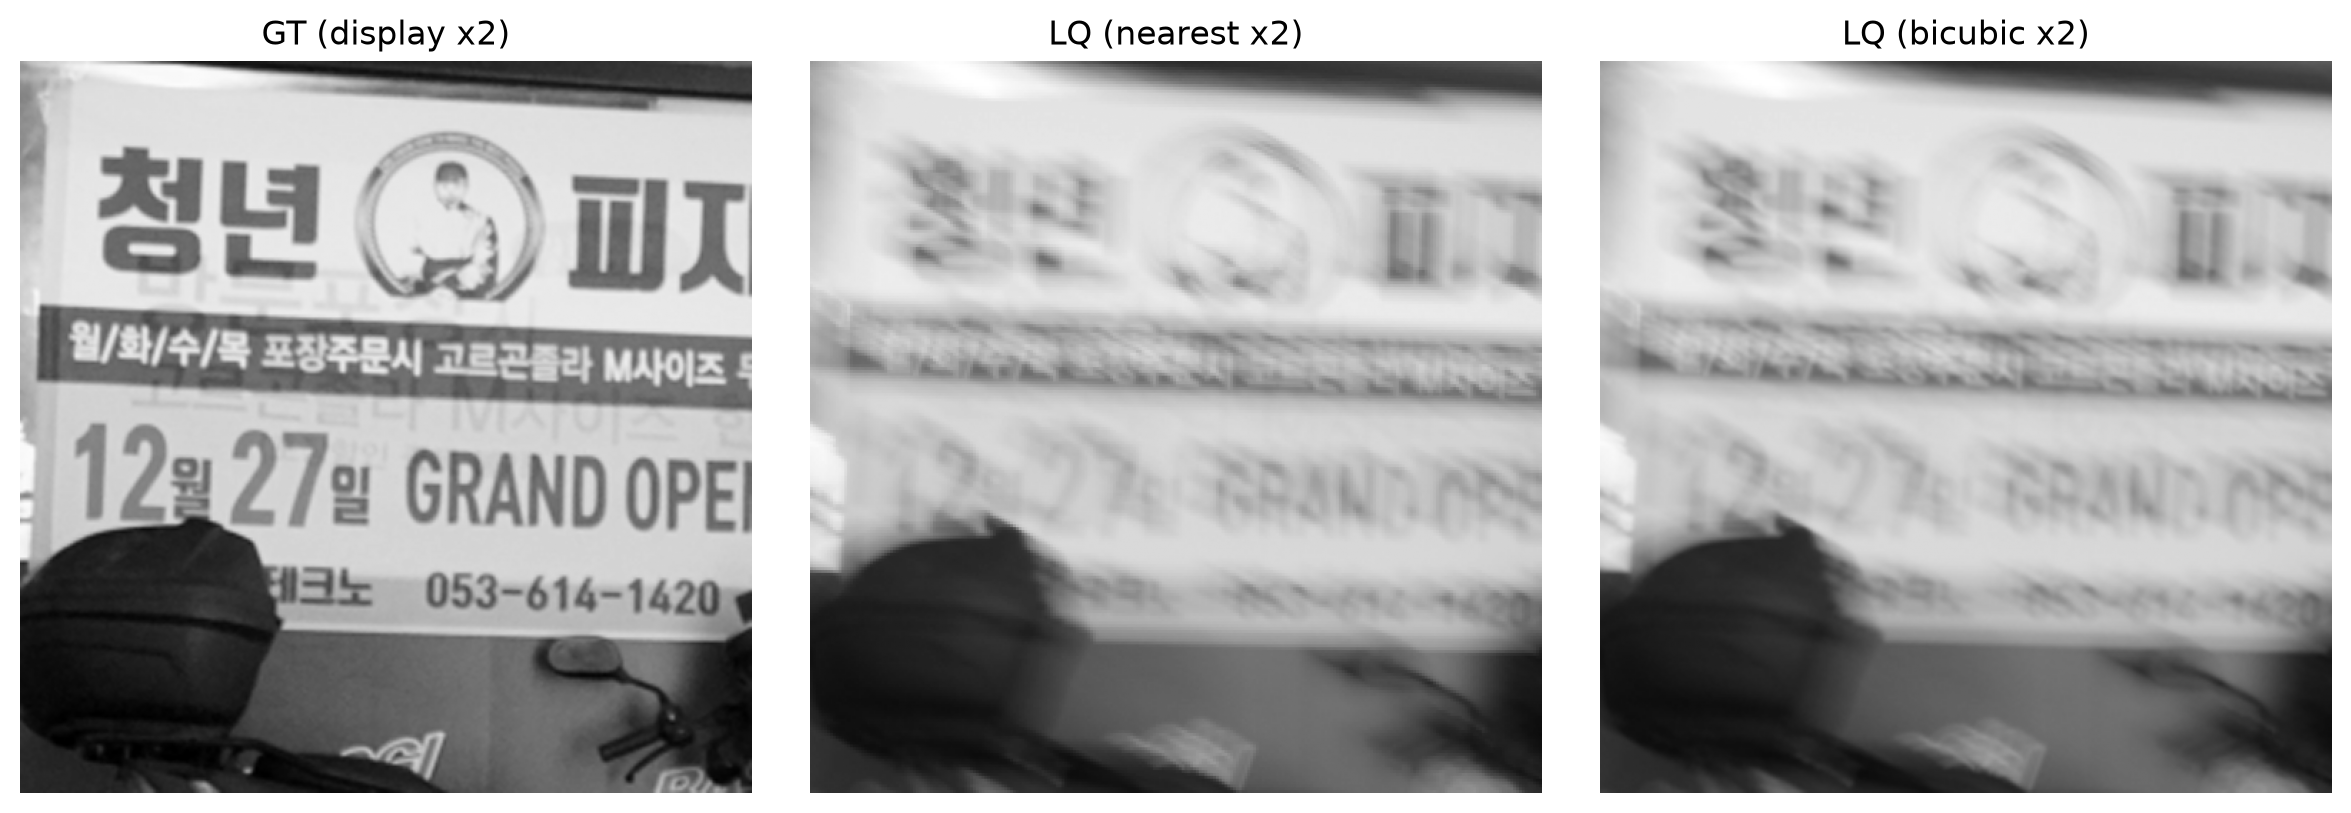
\includegraphics[width=.72\linewidth]{bicubic_x2_comparison.png}
\caption{RealBlur-J 直接双三次放大的显示对照}
\label{fig:bicubic-x2}
\end{figure}

\subsection{RealBlur-J 非局部均值去噪}
NLM 依据局部图像块的相似度对搜索窗口内的像素做加权平均\cite{buades2005nlm}。
实验使用 OpenCV 实现，在 8 位灰度图上固定 \(7\times7\) 模板窗口和
\(21\times21\) 搜索窗口，扫描滤波强度 \(h\)。较大的 \(h\) 允许更多差异较大的块参与平均。
具体调用为 \texttt{fastNlMeansDenoising}，用于测量单纯降噪的效果。

\section{任务四：结果与评价}
\subsection{指标与对比条件}
以同一分支的 GT 和同尺寸结果比较。频域结果在裁剪至 \([0,1]\) 后按浮点值计算。
Bicubic 和 NLM 复用任务三的 8 位处理，评价时统一归一化至 \([0,1]\)。
用 \texttt{scikit-image} 计算 PSNR 和 SSIM，动态范围设为 1（\texttt{data\_range=1.0}）。
设两图有 \(MN\) 个像素，峰值灰度为 1，则
\begin{align}
\mathrm{MSE}&=\frac{1}{MN}\sum_{x,y}(f(x,y)-\widehat f(x,y))^2,&
\mathrm{PSNR}&=10\log_{10}(1/\mathrm{MSE}),\\
\mathrm{SSIM}(a,b)&=
\frac{(2\mu_a\mu_b+C_1)(2\sigma_{ab}+C_2)}
{(\mu_a^2+\mu_b^2+C_1)(\sigma_a^2+\sigma_b^2+C_2)}.&&
\end{align}
SSIM 在局部窗口内比较亮度、对比度及结构，再汇总成全图得分\cite{wang2004ssim}。
局部图使用相同的中心 \(256\times256\) 区域和显示灰度范围。
边界诊断另在最外 16 像素带与内部区域计算 PSNR，并记录浮点裁剪前的越界比例。
PSNR、SSIM 的正式汇总取自任务四 CSV。

\subsection{DIV2K 已知核复原}
表~\ref{tab:div15} 与表~\ref{tab:div19} 按核尺寸汇报三种边界延拓的结果。
两张表的受限逆固定采用各自反射组 PSNR 最好的半径，以便比较同一尺寸内的边界影响。
全部半径中，\(15\times15\) 的反射组在 \(D_0=150\) 两项指标最高，
\(19\times19\) 的反射组在 \(D_0=140\) 时 PSNR 最高，在 \(D_0=180\) 时 SSIM 最高。
% 数据来源：task4/task4_metrics_summary.csv
\begin{table}[htbp]
\centering
\caption{DIV2K $ 15\times15$ 核的边界对照（PSNR（dB）/ SSIM）}
\label{tab:div15}
\begin{tabular}{lccc}
\toprule
方法 & 零填充 & 反射延拓 & 周期延拓 \\
\midrule
LQ & 24.60 / 0.6411 & 24.86 / 0.6433 & 24.75 / 0.6419 \\
全逆滤波 & 5.16 / 0.0031 & 5.16 / 0.0030 & 5.16 / 0.0031 \\
受限逆滤波 $D_0=150$ & 24.92 / 0.6776 & 25.24 / 0.6764 & 25.71 / 0.6980 \\
Wiener $K=0.01$ & 26.14 / 0.7783 & 26.86 / 0.7788 & 27.35 / 0.7858 \\
CLS $\gamma=0.01$ & 25.74 / 0.7718 & 26.39 / 0.7720 & 27.64 / 0.7850 \\
Bicubic Down-Up & 24.69 / 0.6591 & 24.94 / 0.6614 & 24.83 / 0.6600 \\
\bottomrule
\end{tabular}
\end{table}

% 数据来源：task4/task4_metrics_summary.csv
\begin{table}[htbp]
\centering
\caption{DIV2K $ 19\times19$ 核的边界对照（PSNR（dB）/ SSIM）}
\label{tab:div19}
\begin{tabular}{lccc}
\toprule
方法 & 零填充 & 反射延拓 & 周期延拓 \\
\midrule
LQ & 24.52 / 0.6368 & 24.78 / 0.6390 & 24.66 / 0.6376 \\
全逆滤波 & 5.30 / 0.0040 & 5.30 / 0.0039 & 5.30 / 0.0040 \\
受限逆滤波 $D_0=140$ & 24.74 / 0.6609 & 25.06 / 0.6608 & 25.33 / 0.6751 \\
Wiener $K=0.01$ & 26.15 / 0.7804 & 26.86 / 0.7808 & 27.39 / 0.7875 \\
CLS $\gamma=0.01$ & 25.79 / 0.7739 & 26.42 / 0.7740 & 27.68 / 0.7862 \\
Bicubic Down-Up & 24.60 / 0.6549 & 24.85 / 0.6572 & 24.74 / 0.6557 \\
\bottomrule
\end{tabular}
\end{table}

\FloatBarrier

两种核尺寸的反射组中，固定 \(K=0.01\) 的 Wiener 较 LQ 分别提高约 \(2.00\) 和 \(2.09\) dB。
双三次 Down-Up 约提高 \(0.08\) dB，边缘仍保留 LQ 的模糊。
图~\ref{fig:divfull} 和图~\ref{fig:divcrop} 分别展示 \(15\times15\) 反射组的全图与中心区域。
\begin{figure}[H]
\centering
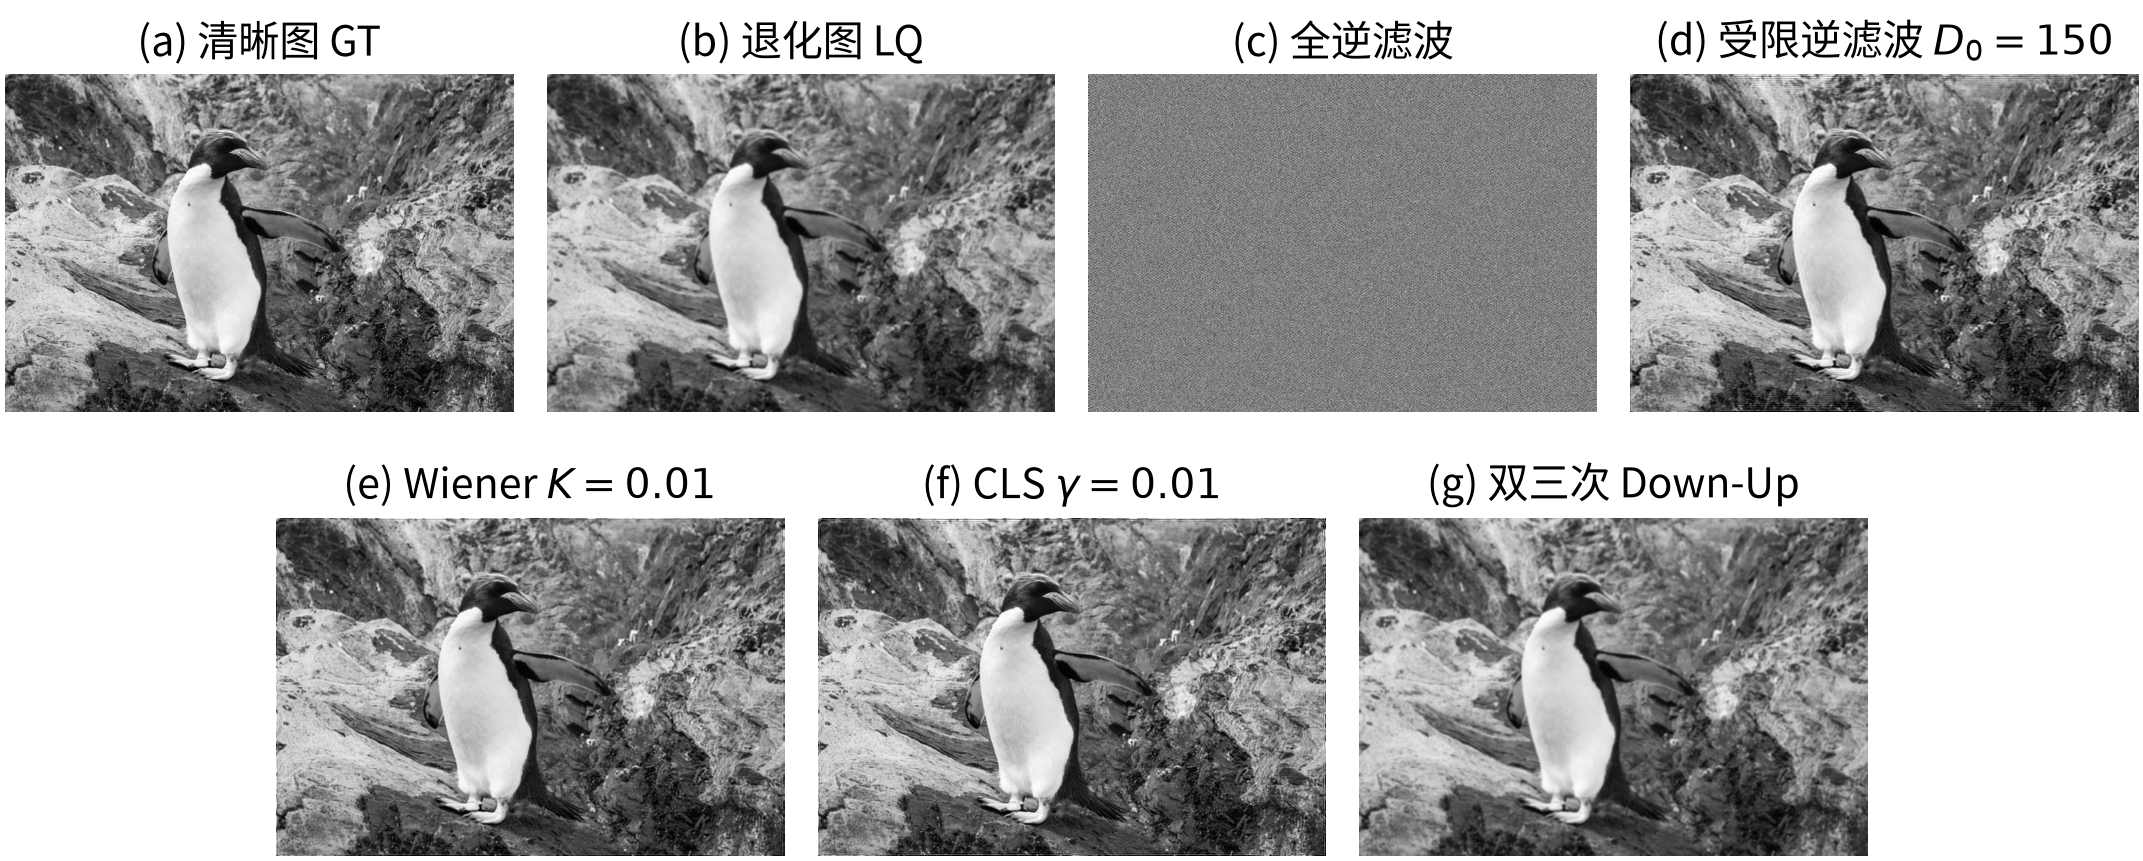
\includegraphics[width=\linewidth]{div2k_reflect_full.png}
\caption{DIV2K \(15\times15\) 反射延拓组全图的复原与对照}
\label{fig:divfull}
\end{figure}
\begin{figure}[H]
\centering
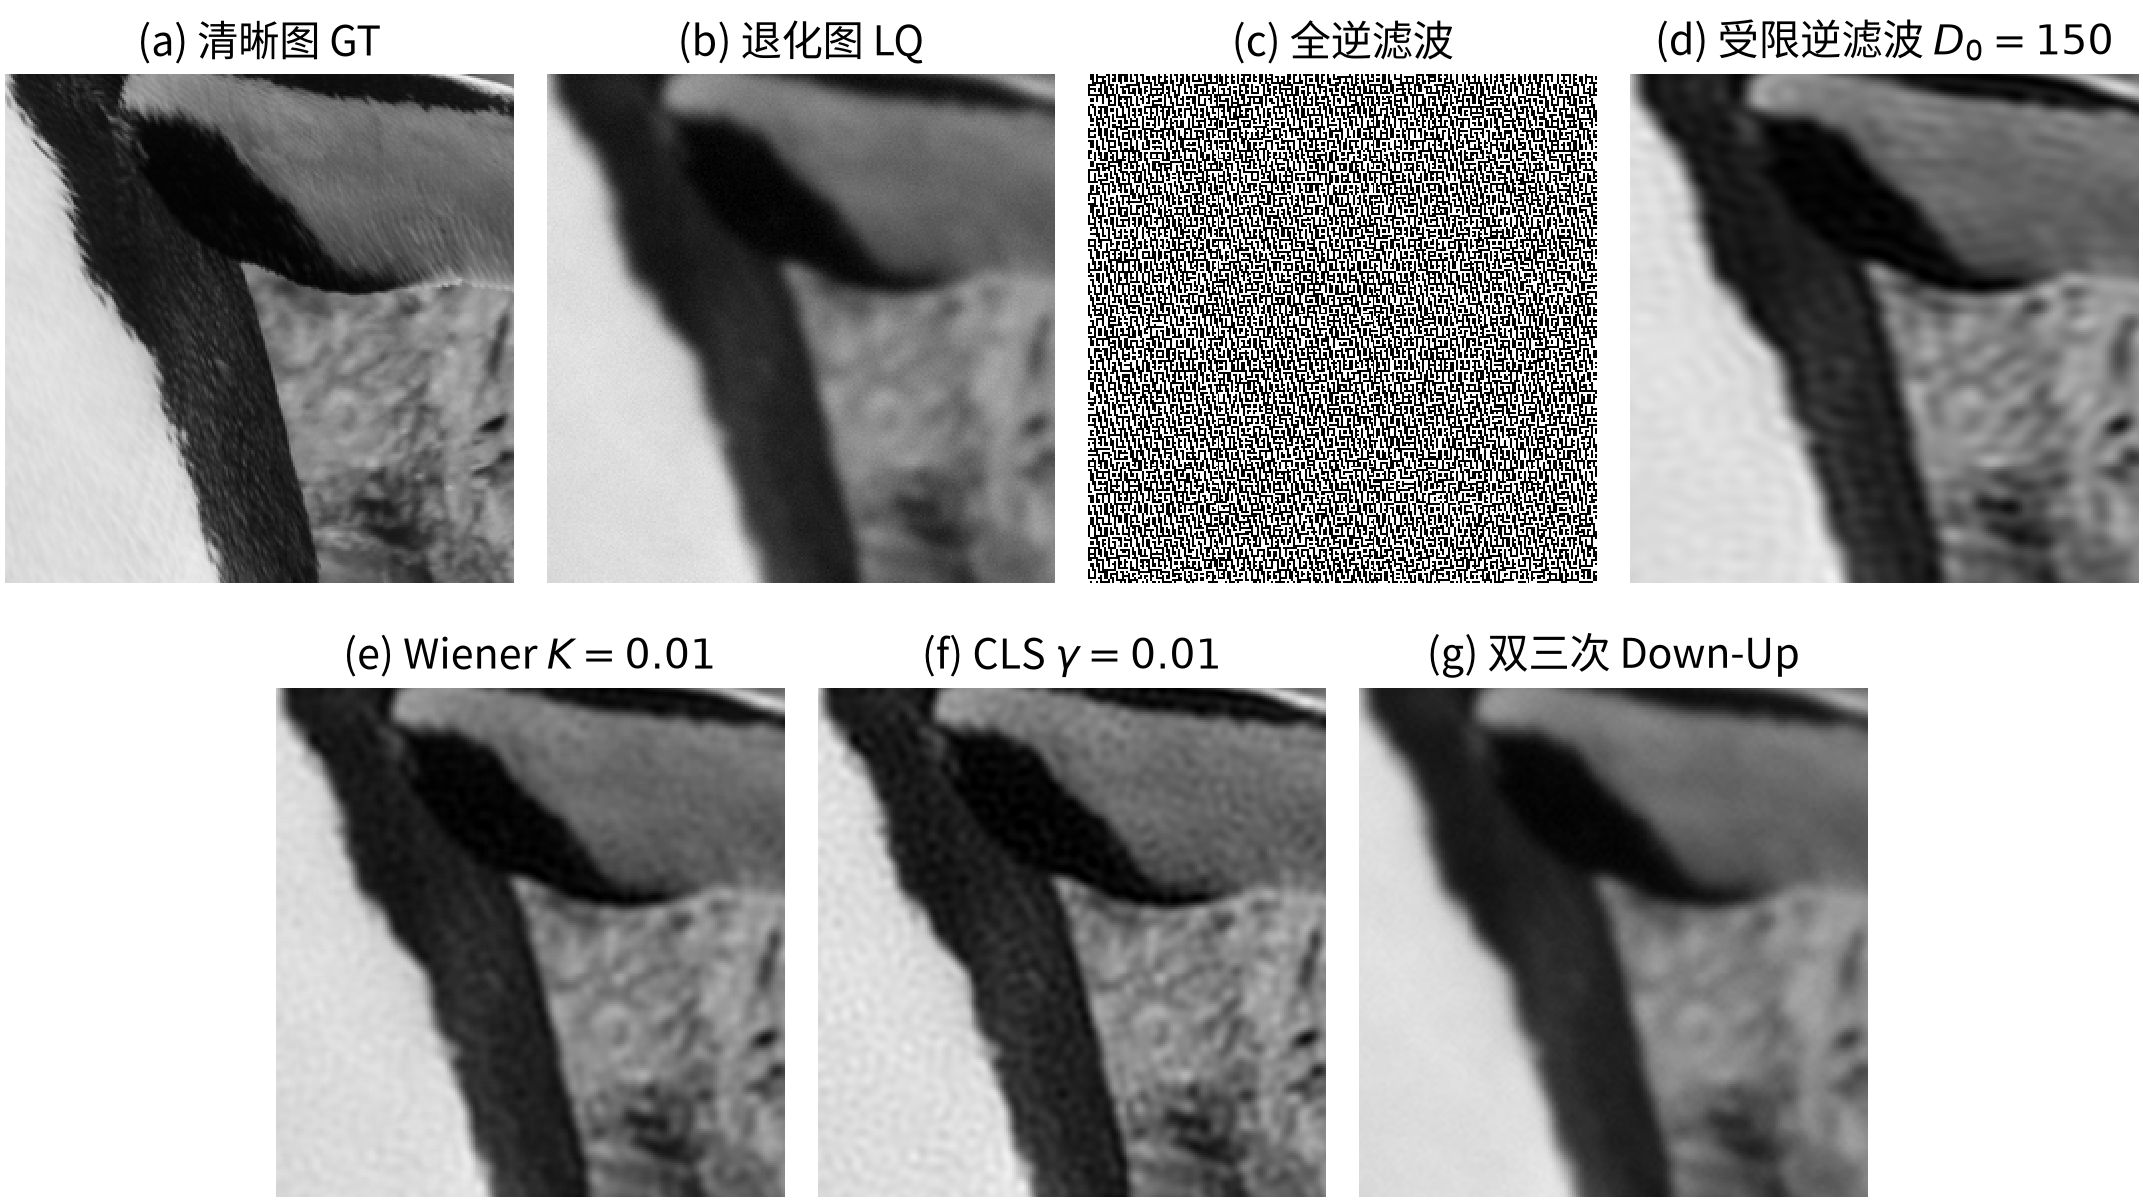
\includegraphics[width=\linewidth]{div2k_reflect_crop.png}
\caption{DIV2K \(15\times15\) 反射延拓组中心区域的复原与对照}
\label{fig:divcrop}
\end{figure}
LQ 中企鹅轮廓发软，全逆出现密集黑白噪点。
受限逆找回一部分轮廓，Wiener 和 CLS 进一步加强了轮廓与岩石纹理，细羽毛与 GT 仍有差别。

\Needspace{.64\textheight}
图~\ref{fig:boundary} 将 LQ、Wiener、CLS 的全图按边界方式并列。
两种核尺寸下，周期组的 Wiener 较反射组提高 \(0.49\)--\(0.52\) dB，CLS 提高 \(1.25\)--\(1.27\) dB。
例如 \(15\times15\) 组的 Wiener 边界带 PSNR 从 20.473 提高至 24.754 dB，
内部均约为 27.5 dB，收益集中在边界。周期组中 CLS 的 PSNR 最高，Wiener 的 SSIM 最高。
结论适用于当前退化图和循环卷积实现。
\begin{figure}[H]
\centering
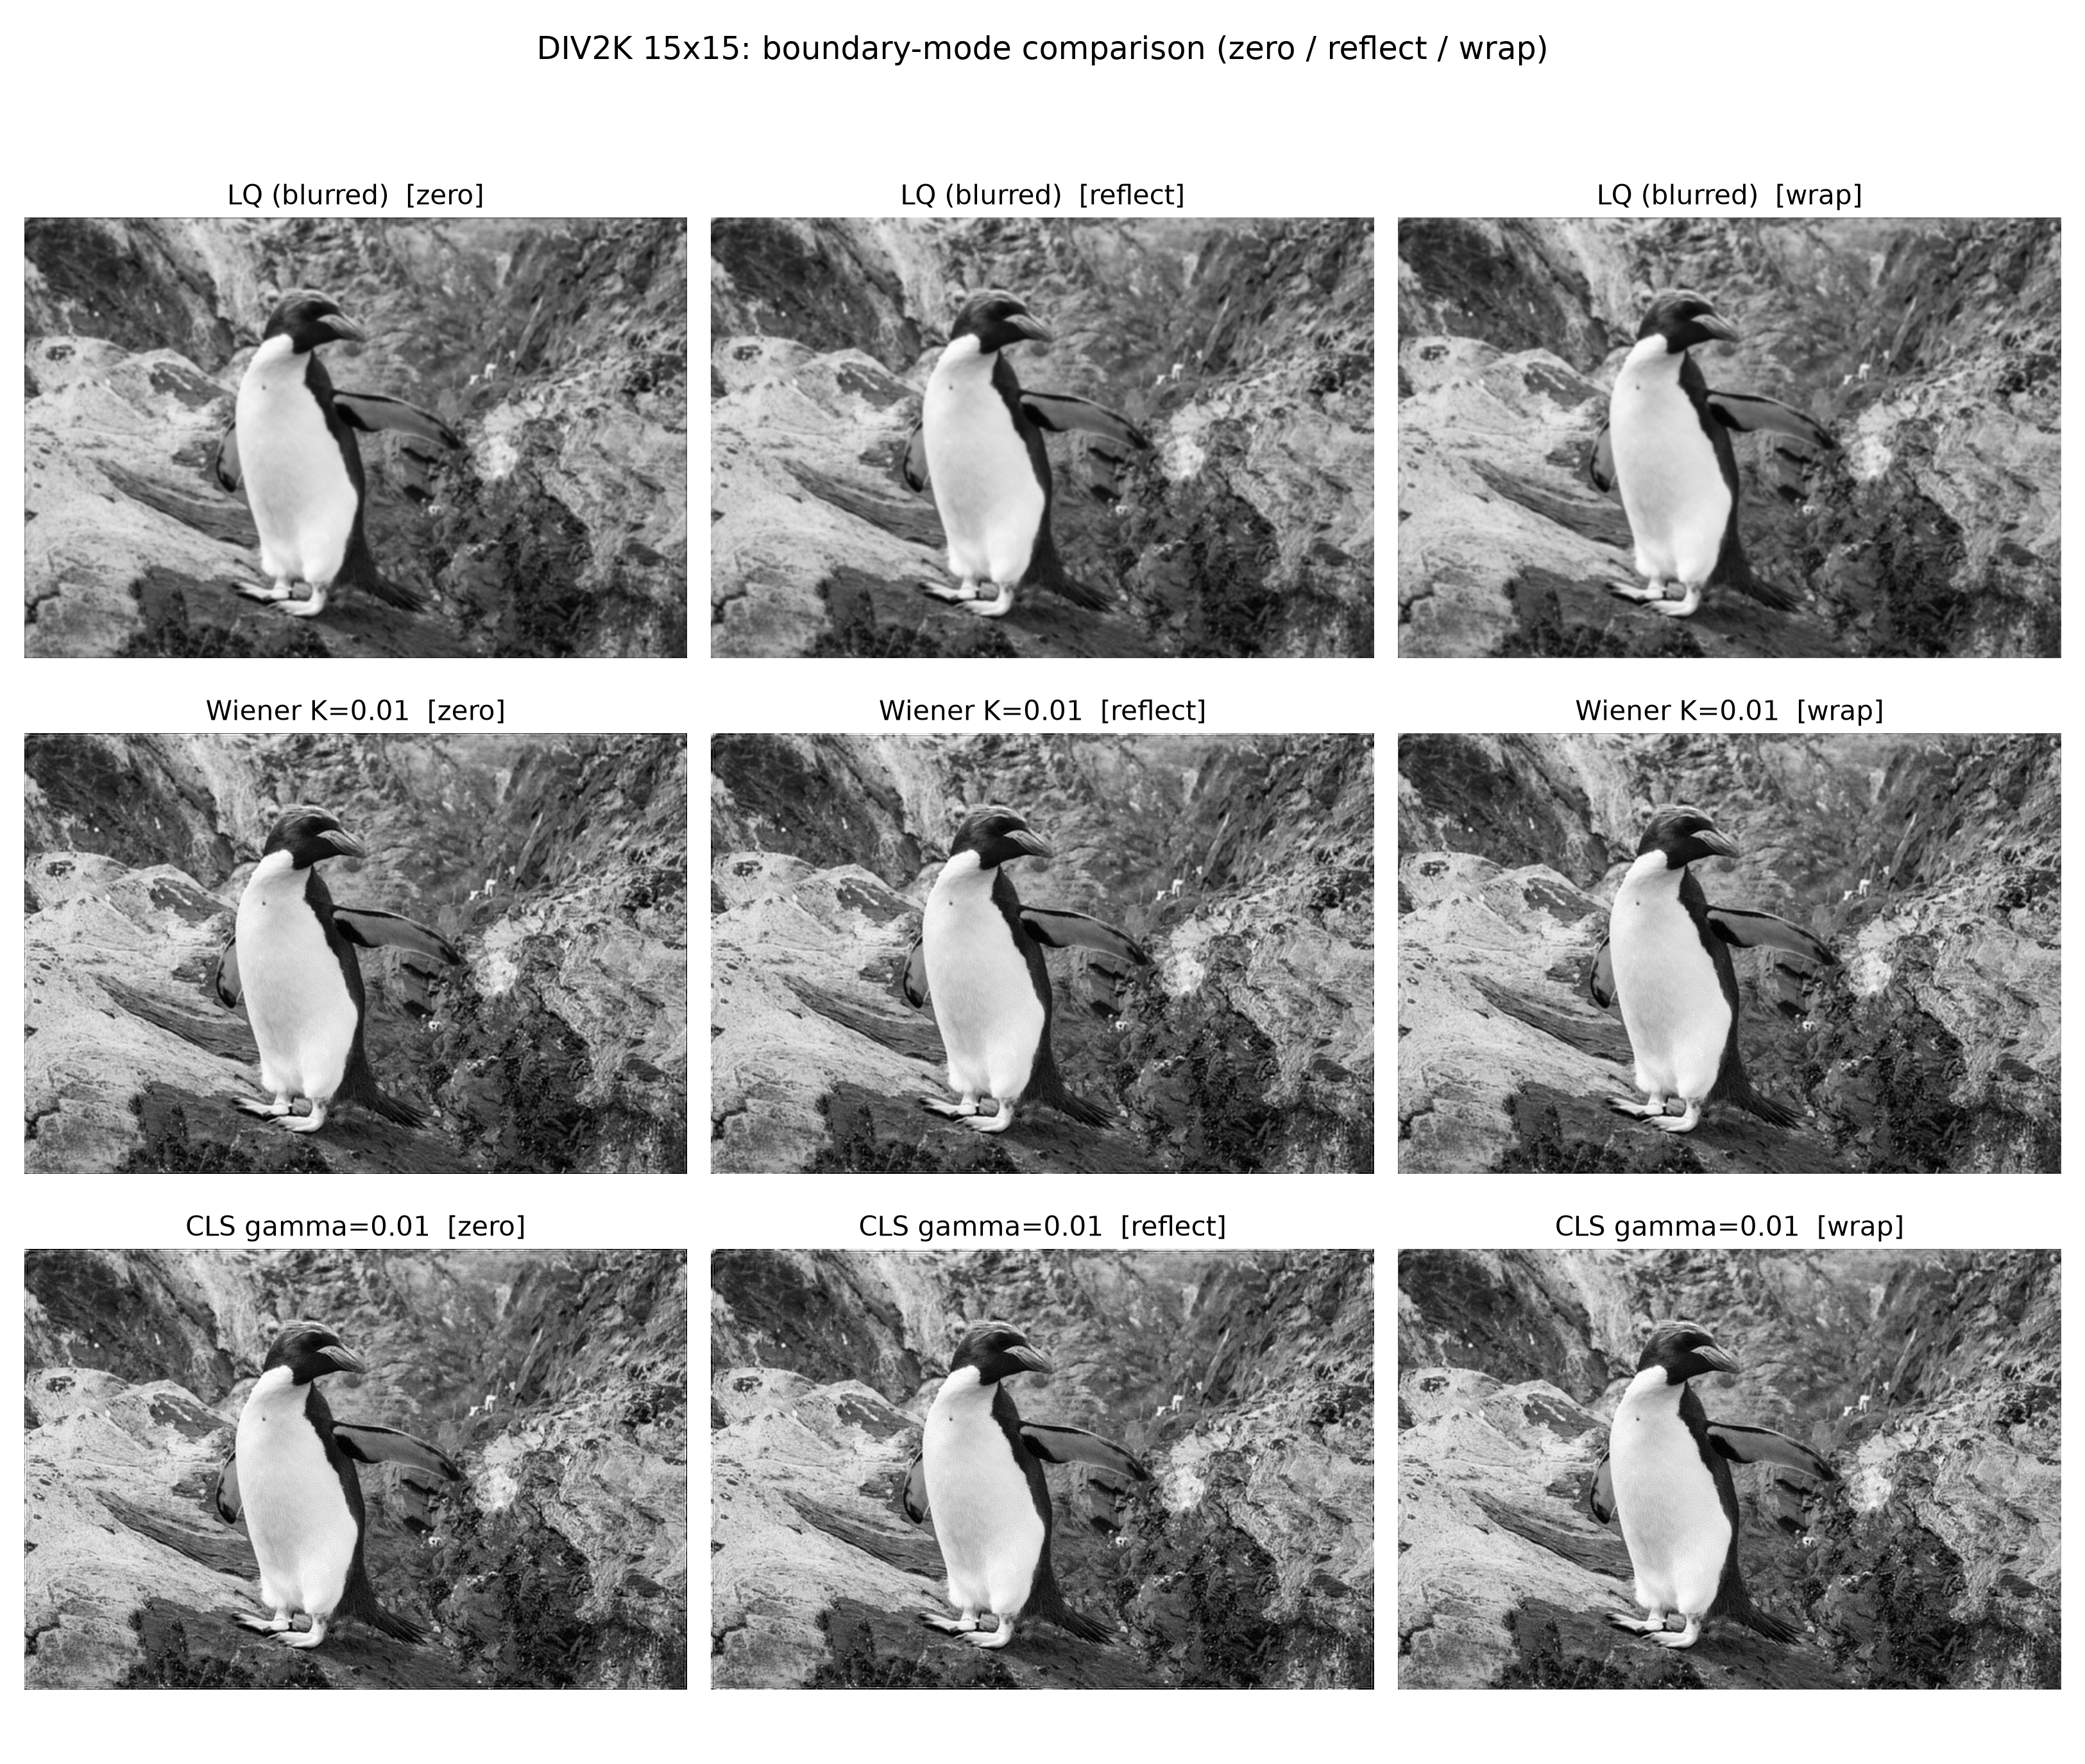
\includegraphics[width=.73\linewidth]{div2k_15x15_boundary_compare.png}
\caption{DIV2K \(15\times15\) 全图边界对照。行依次为 LQ、Wiener、CLS，列依次为零填充、反射延拓、周期延拓}
\label{fig:boundary}
\end{figure}

\subsection{RealBlur-J 高斯猜核与对照}
固定 \(\sigma=3\) 比较 \(15\times15\) 与 \(35\times35\) 核，再固定 \(35\times35\) 比较 \(\sigma=3,5,7\)。
表~\ref{tab:rb-gauss} 展示四种高斯假设，表~\ref{tab:rb-controls} 展示原始 LQ 与两类对照。
本组固定的 \(K=\gamma=0.01\) 及所测各档 \(D_0\) 下，所有高斯猜核复原的两项指标均低于 LQ。
最好的受限逆 PSNR 为 18.7930 dB（\(35\times35,\ \sigma=3,\ D_0=30\)），
而最高 SSIM 为 0.51214（\(15\times15,\ \sigma=3,\ D_0=30\)）。
NLM 扫描中 \(h=8\) 的 PSNR 最高，\(h=13\) 的 SSIM 最高。
% 数据来源：task4/task4_metrics_summary.csv
\begin{table}[htbp]
\centering
\footnotesize
\setlength{\tabcolsep}{4pt}
\caption{RealBlur-J 高斯假设核复原结果（PSNR（dB）/ SSIM）}
\label{tab:rb-gauss}
\begin{tabular}{lcccc}
\toprule
假设核 & 全逆滤波 & 受限逆 $D_0=30$ & Wiener $K=0.01$ & CLS $\gamma=0.01$ \\
\midrule
$ 15\times15$，$\sigma=3$ & 4.77 / 0.0027 & 18.79 / 0.5121 & 17.49 / 0.4463 & 16.33 / 0.3625 \\
$ 35\times35$，$\sigma=3$ & 5.37 / 0.0077 & 18.79 / 0.5112 & 17.44 / 0.4481 & 16.31 / 0.3669 \\
$ 35\times35$，$\sigma=5$ & 5.10 / 0.0100 & 18.64 / 0.4777 & 16.45 / 0.3999 & 12.43 / 0.1812 \\
$ 35\times35$，$\sigma=7$ & 4.77 / 0.0032 & 17.36 / 0.3855 & 16.50 / 0.4010 & 9.27 / 0.0996 \\
\bottomrule
\end{tabular}
\end{table}

% 数据来源：task4/task4_metrics_summary.csv
\begin{table}[htbp]
\centering
\caption{RealBlur-J 输入与插值、去噪对照}
\label{tab:rb-controls}
\begin{tabular}{lrr}
\toprule
方法 & PSNR（dB） & SSIM \\
\midrule
LQ & 18.9246 & 0.57394 \\
Bicubic Down-Up & 18.9500 & 0.57565 \\
NLM $h=8$ & 18.9469 & 0.58211 \\
NLM $h=13$ & 18.9332 & 0.58268 \\
\bottomrule
\end{tabular}
\end{table}

\FloatBarrier

图~\ref{fig:rbfull} 给出全图结果，图~\ref{fig:rbcrop} 放大了招牌中心区域。
\begin{figure}[H]
\centering
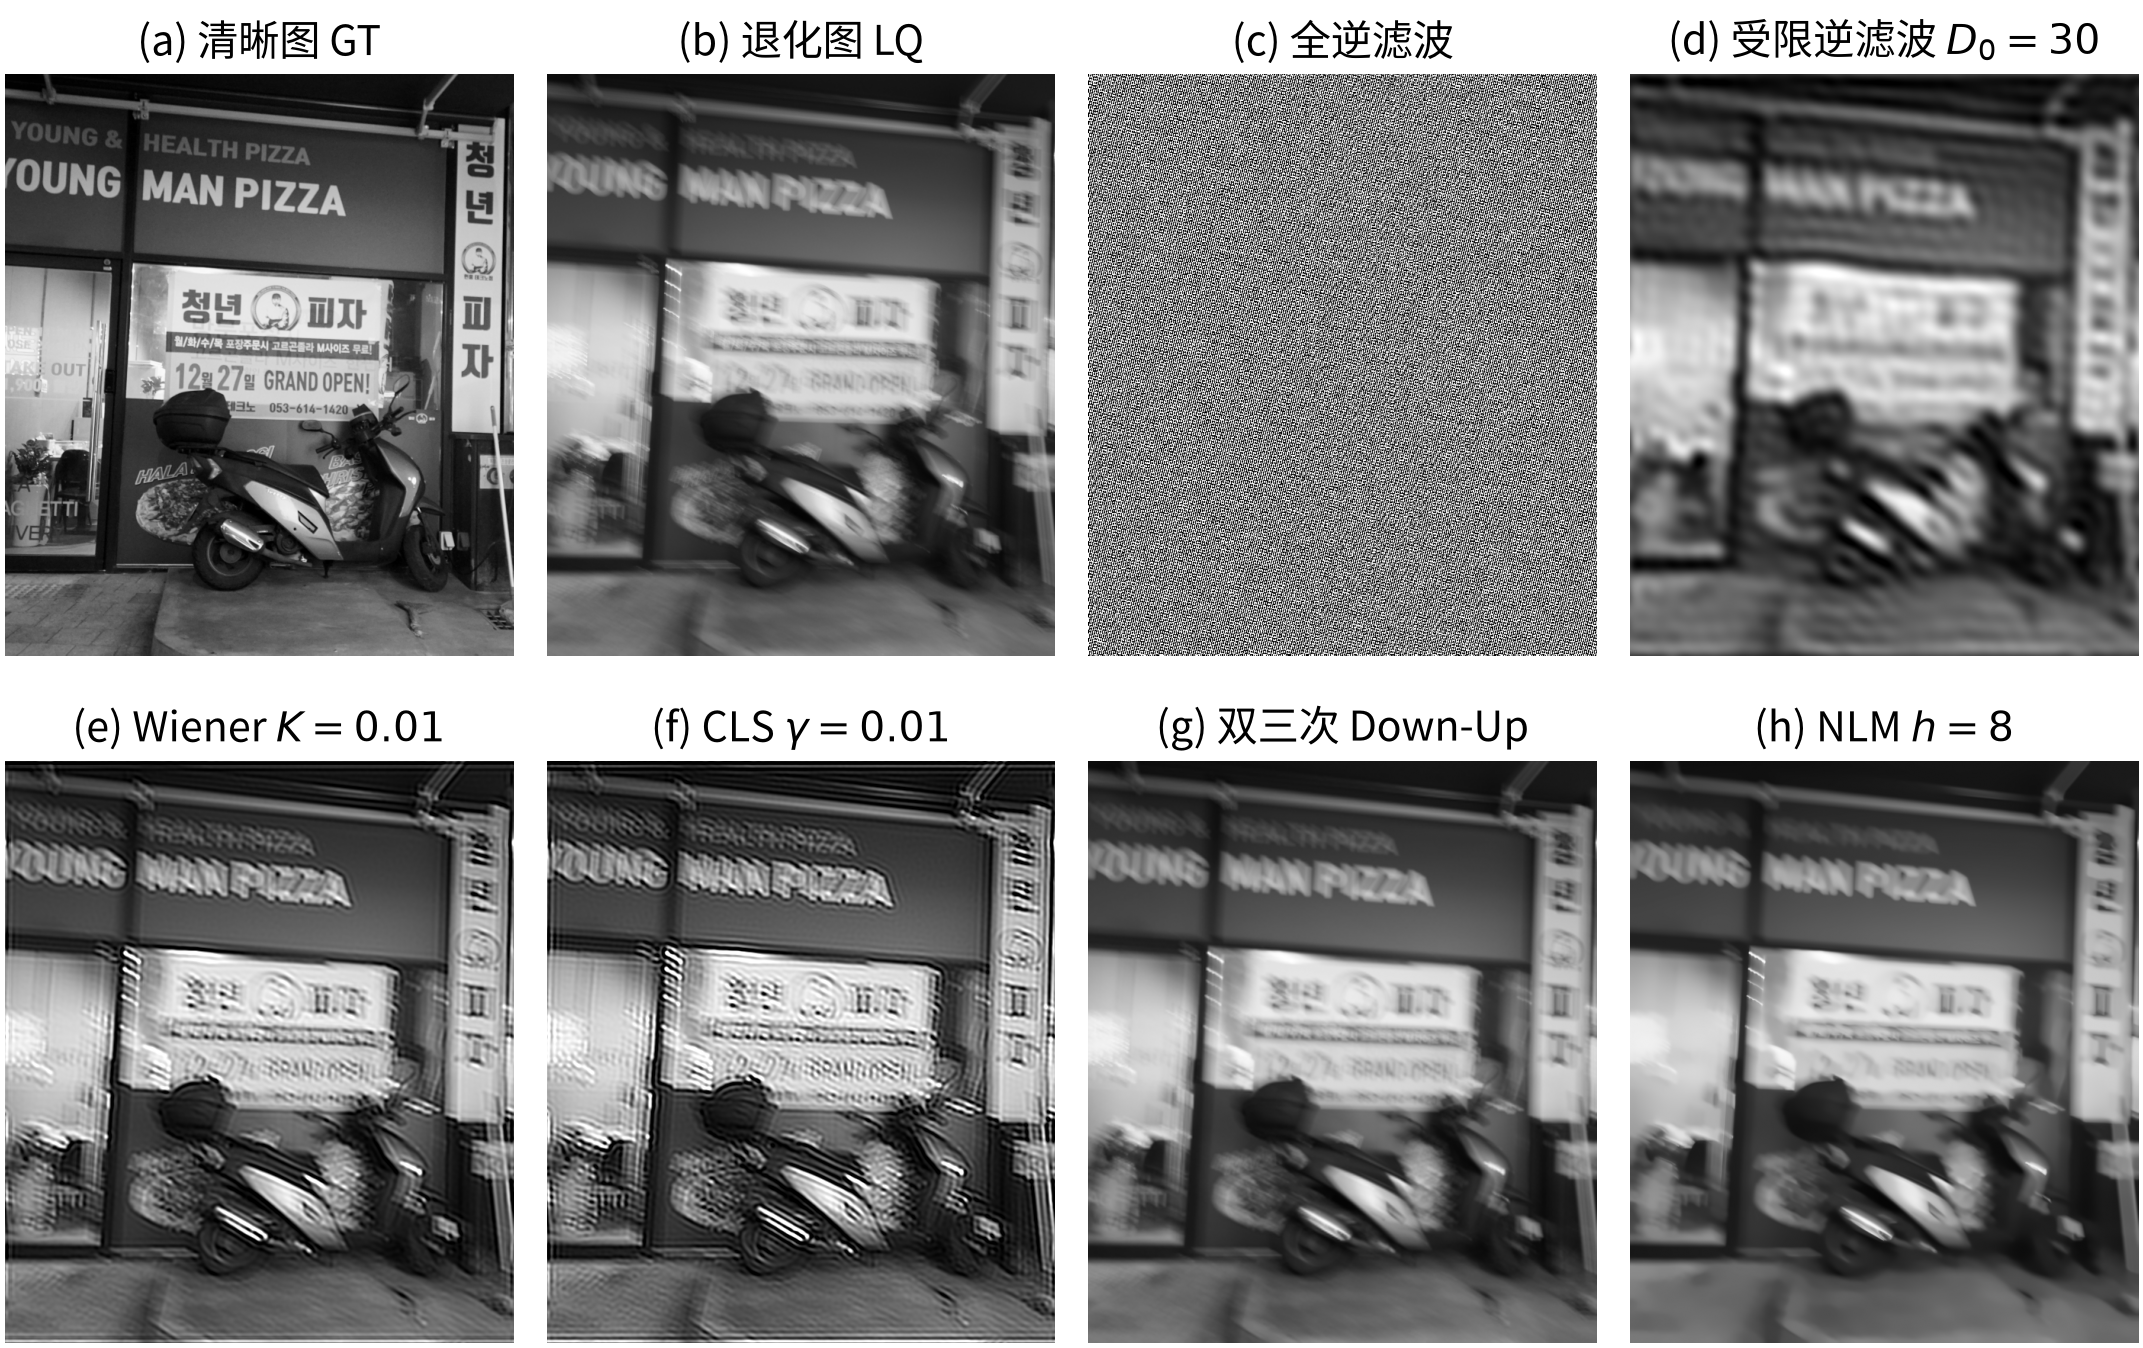
\includegraphics[width=.94\linewidth]{realblur_full.png}
\caption{RealBlur-J 全图的复原与对照}
\label{fig:rbfull}
\end{figure}
\begin{figure}[H]
\centering
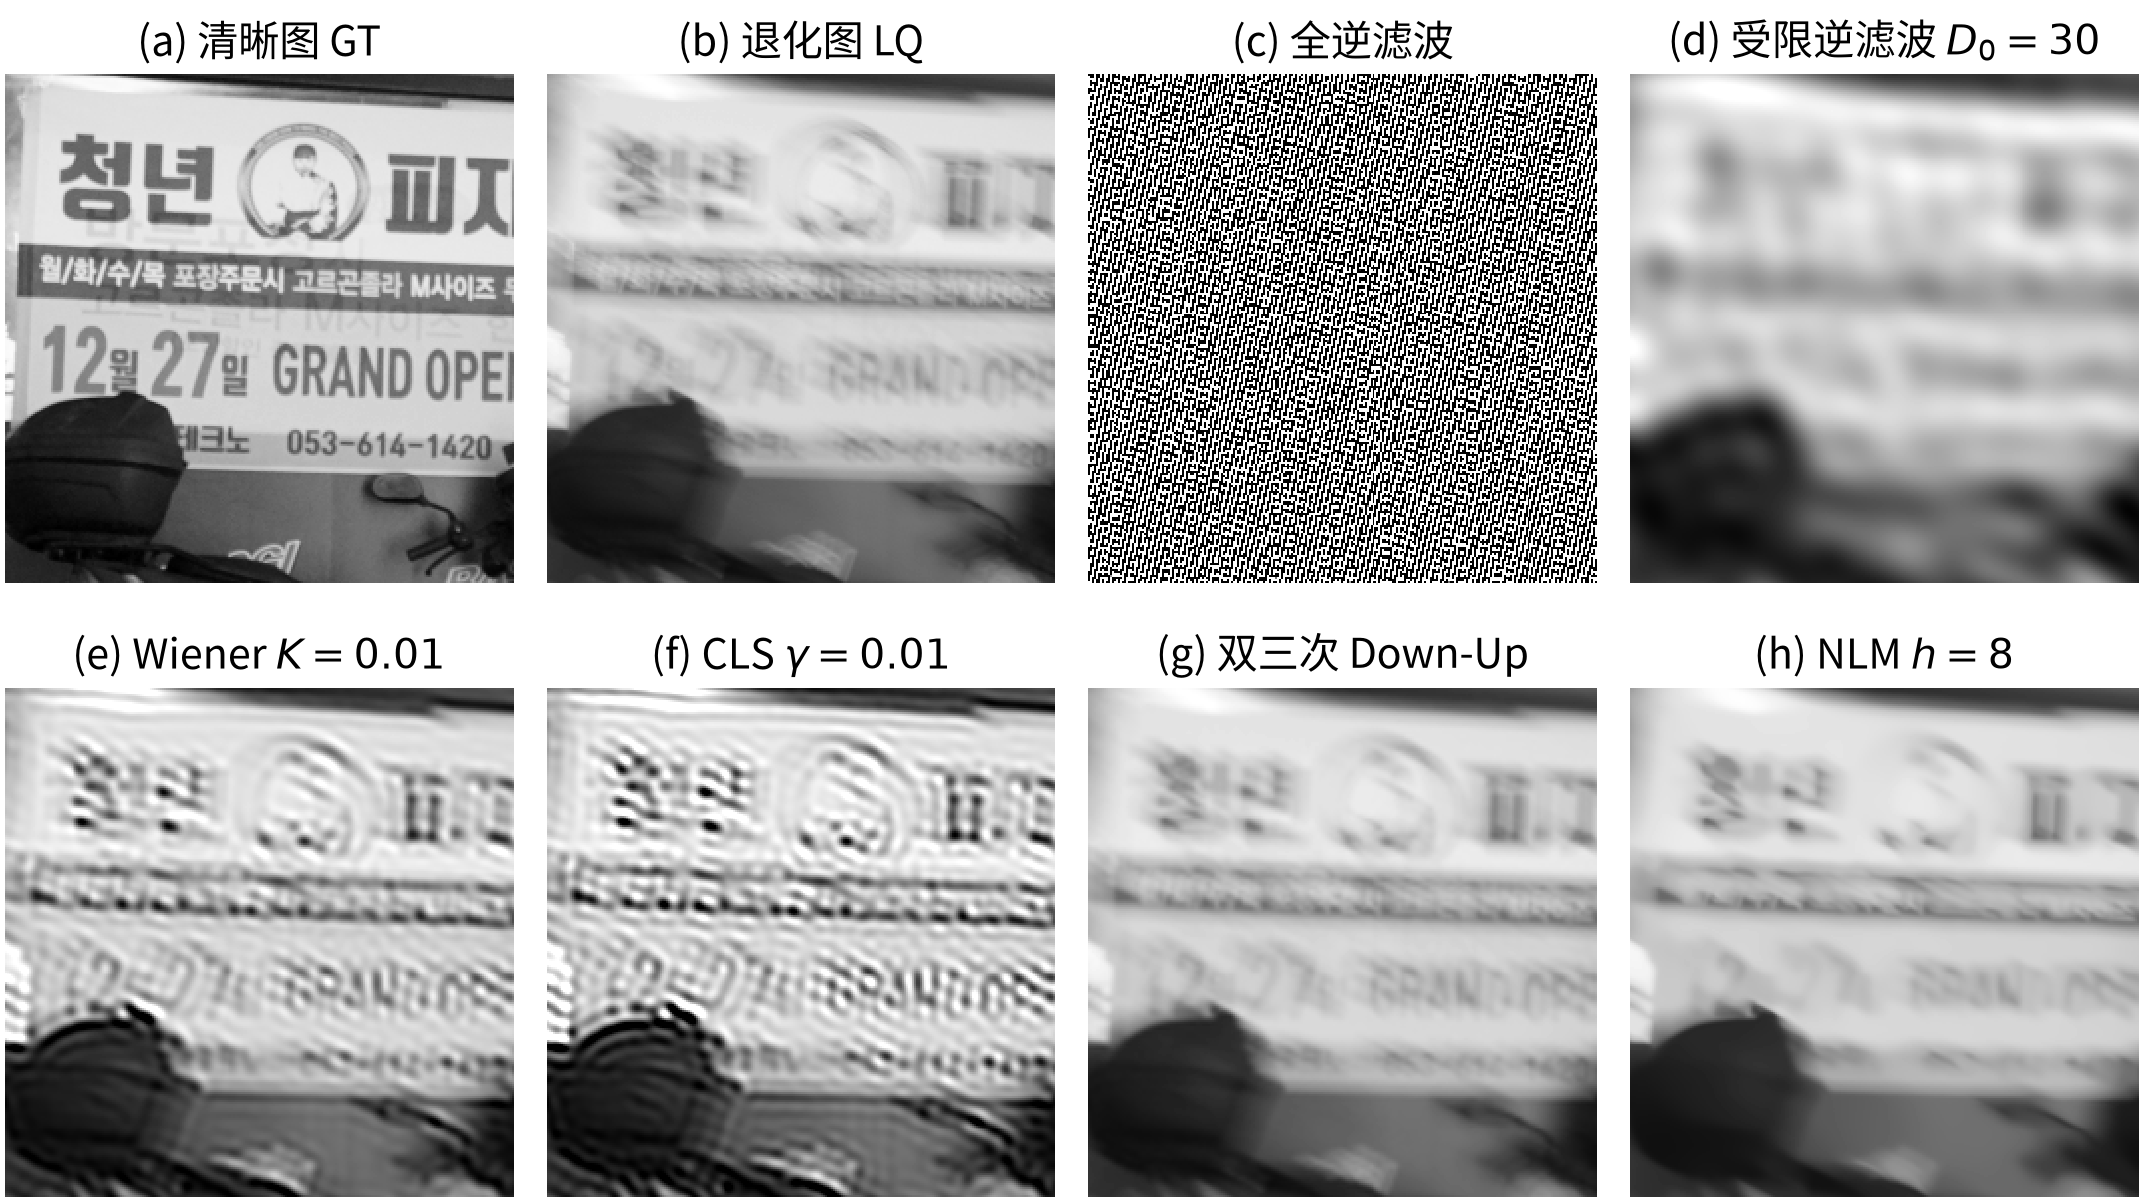
\includegraphics[width=\linewidth]{realblur_crop.png}
\caption{RealBlur-J 招牌中心区域。频域主实验使用 \(15\times15,\ \sigma=3\) 高斯猜核，去噪展示 \(h=8\)}
\label{fig:rbcrop}
\end{figure}
全逆结果几乎被噪声覆盖，受限逆保留了招牌的低频轮廓。
采用 \(15\times15,\ \sigma=3\) 的高斯核后，Wiener 与 CLS 使笔画和招牌边沿出现亮暗重复轮廓。
Bicubic 和 NLM 略微平滑了局部变化，招牌的运动拖尾仍可见。

\Needspace{6\baselineskip}
\section{任务五：实验分析}
\subsection{逆滤波为何失效}
由 \(\widehat F=F+N/H\) 可见，退化已经压低的频率分量会以 \(1/|H|\) 成比例放大噪声。
DIV2K \(15\times15\) 反射组的全逆只有 5.1594 dB，约 \(99.947\%\) 像素在裁剪前越界。
\(D_0=30\) 的受限逆舍弃大量有效频率，PSNR 为 19.4911 dB。
扩大到 150 可提高到 25.2432 dB，扩大到 200 又降到 22.2133 dB。
硬频率截止的空域冲激响应还有振荡旁瓣，强边缘附近可能出现振铃。

\subsection{正则化与信噪比的取舍}
表~\ref{tab:param} 固定 \(15\times15\) 反射组的 LQ 和 PSF，各扫描六档 \(K,\gamma\)。
\(K=0.0001\) 时 Wiener 接近弱约束逆滤波，PSNR 只有 15.0451 dB。
提高到 \(0.01\) 时，两项指标最高，进一步升至 \(0.1\) 后，PSNR 降至 23.0340 dB。
CLS 两项指标在 \(\gamma=0.05\) 最高。升至 \(0.1\) 后 PSNR 和 SSIM 分别下降约 0.072 dB 和 0.00858。
当前样本的扫描表现为末端温和下降。模型表明继续增大 \(\gamma\) 会更强地压制真实边缘与细纹理。
跨分支比较仍采用预设的 \(\gamma=0.01\)，参数扫描用于考察该样本的调节范围。
图~\ref{fig:params} 显示两种方法的 PSNR 峰值位置。
% 数据来源：task2/param/param_fixed/task2_parameter_metrics.csv
\begin{table}[H]
\centering
\caption{DIV2K $15\times15$ 反射延拓组的参数扫描}
\label{tab:param}
\begin{tabular}{crrrr}
\toprule
参数值（$K$ 或 $\gamma$） & Wiener PSNR（dB） & Wiener SSIM & CLS PSNR（dB） & CLS SSIM \\
\midrule
0.0001 & 15.0451 & 0.18176 & 18.0373 & 0.31062 \\
0.001 & 23.6781 & 0.63985 & 23.2108 & 0.62870 \\
0.005 & 26.6415 & 0.77292 & 25.7932 & 0.75102 \\
0.01 & 26.8605 & 0.77884 & 26.3865 & 0.77200 \\
0.05 & 25.3034 & 0.73943 & 26.8294 & 0.77795 \\
0.1 & 23.0340 & 0.70339 & 26.7573 & 0.76937 \\
\bottomrule
\end{tabular}
\end{table}

\begin{figure}[H]
\centering
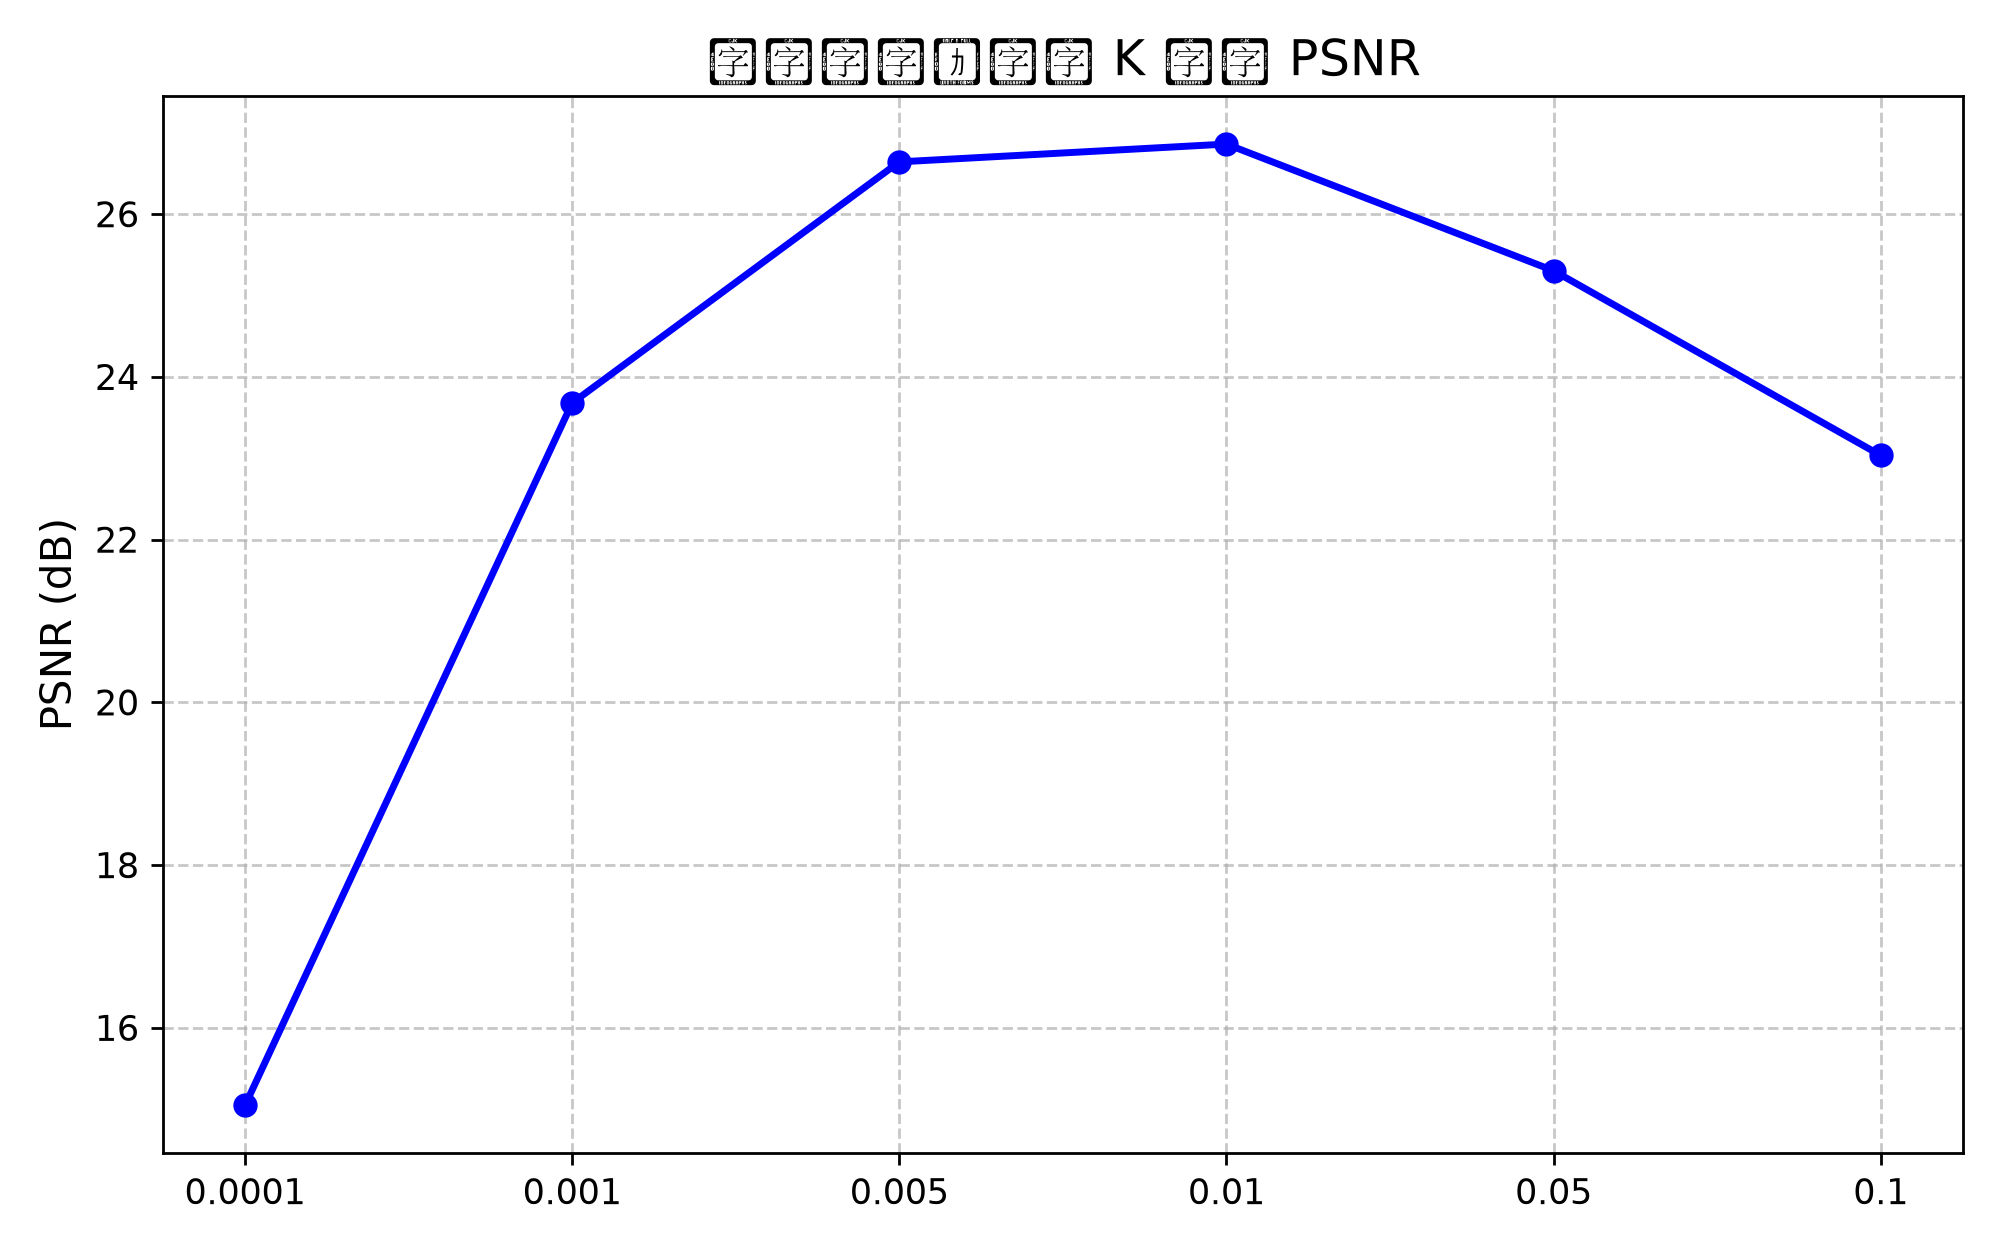
\includegraphics[width=.47\linewidth]{1_wiener_psnr.png}\hfill
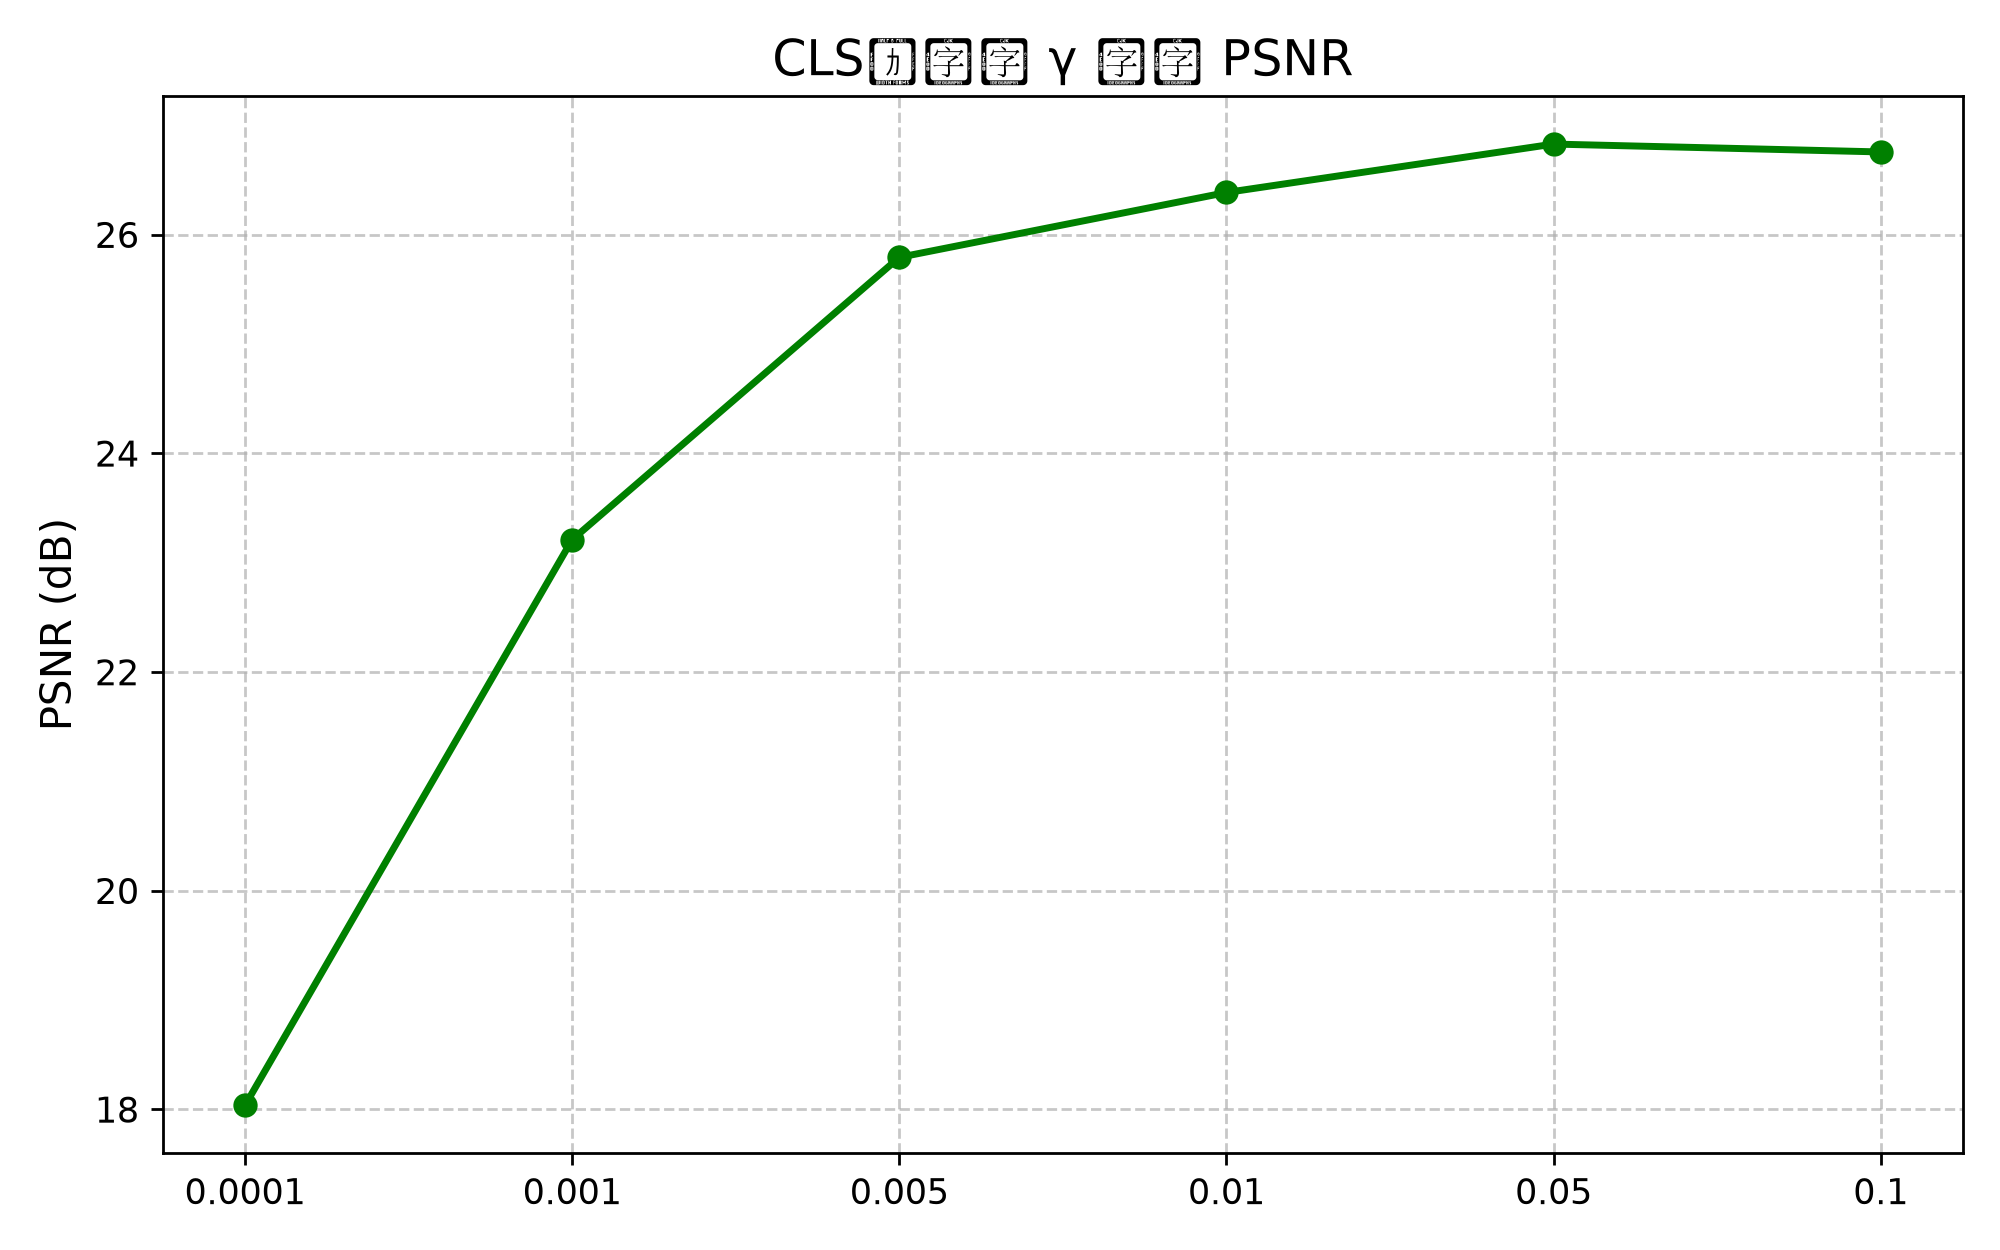
\includegraphics[width=.47\linewidth]{3_cls_psnr.png}
\caption{DIV2K \(15\times15\) 反射延拓组的参数扫描，两图横坐标为离散候选值}
\label{fig:params}
\end{figure}

\subsection{空间不变假设与核失配}
DIV2K 用已知高斯 PSF 合成数据，图像内部的退化与复原使用同一个核。周期组还满足 FFT 的边界假设。
对实拍模糊，不同位置可能具有不同的轨迹和拖尾，单个全局 PSF 只能近似。
若真实系统可局部以频率响应 \(H_t\) 近似，而复原采用 \(H_a\)，理想逆滤波的误差为
\begin{equation}
\widehat F-F=\left(\frac{H_t}{H_a}-1\right)F+\frac{N}{H_a}.
\end{equation}
第一项显示即使无噪声，错核也会引起与原图相关的误差。
高斯核各向同性，真实运动核往往有方向性，两者的衰减频率和零点可不同。
错误补偿使等效响应出现振荡，在笔画和边沿产生过冲、欠冲及重复轮廓。
核未知的盲复原还需从观测中估计退化，清晰图与核的多种组合可能解释同一 LQ，通常需要额外的核或图像先验。

\subsection{复原与插值的作用}
去卷积根据 PSF 和噪声模型估计清晰图，修正受衰减的频率成分。双三次插值根据邻域估计新网格的灰度，
可改善显示尺寸与连续性。Down-Up 的小幅指标改善可来自重采样平滑，与去卷积的模型反演不同。
NLM 利用块自相似抑制局部噪声，本实验中的实拍拖尾仍然保留。
\FloatBarrier

\section{选做：Radon 运动核估计}
近似匀速直线运动对应有方向的线状 PSF，傅里叶幅度沿运动方向的频率剖面具有条纹与谷值。
程序在 LQ 的中心方形区域去均值并加 Hann 窗，增强对数幅度谱中相对背景较暗的条纹，
在 \(0^\circ\) 至 \(179^\circ\) 的 Radon 投影上按变化强度寻找主方向，
再在估计方向附近对平行频谱剖面取平均，用最显著谷值至频谱中心的距离近似第一零点。
若边长为 \(n\)、距离为 \(d\) 个频率格点，则以 \(n/d\) 估计长度并构造归一化直线 PSF。
显著谷值可能对应更高阶的零点，因而长度估计是启发式的。
在同一 DIV2K 图像的七个合成设置上（表~\ref{tab:radon-synthetic}），所测角度的绝对误差均为 \(0^\circ\)，长度平均绝对误差约 1.30 像素，
最大为 3.11 像素。使用估计核的 Wiener 结果在七组中均提高了 PSNR。
% 数据来源：task3_extra/output/synthetic_summary.csv
\begin{table}[htbp]
\centering
\caption{合成直线运动模糊的方向与长度估计}
\label{tab:radon-synthetic}
\begin{tabular}{rrrrr}
\toprule
真实方向（$^\circ$） & 估计方向（$^\circ$） & 真实长度（px） & 估计长度（px） & 长度绝对误差（px） \\
\midrule
0 & 0 & 23 & 24.38 & 1.38 \\
30 & 30 & 23 & 22.26 & 0.74 \\
60 & 60 & 23 & 21.33 & 1.67 \\
90 & 90 & 23 & 22.26 & 0.74 \\
30 & 30 & 12 & 11.13 & 0.87 \\
30 & 30 & 40 & 39.38 & 0.62 \\
30 & 30 & 60 & 56.89 & 3.11 \\
\bottomrule
\end{tabular}
\end{table}


RealBlur-J 样本的估计方向与长度约为 \(29^\circ\) 和 26.95 像素。
表~\ref{tab:radon} 显示同一个核在不同正则化设置下的表现。\(K=0.10\) 的 PSNR 最高，
\(K=0.15\) 的 SSIM 最高，二者均相对原始 LQ 有改善。
核估计只使用 LQ，GT 用于复原评价和事后参数扫描。真实核的角度和长度没有真值用于验证。
% 数据来源：task4/task4_metrics_summary.csv
\begin{table}[htbp]
\centering
\caption{RealBlur-J 估计运动核的复原结果}
\label{tab:radon}
\begin{tabular}{lrr}
\toprule
方法 & PSNR（dB） & SSIM \\
\midrule
Wiener $K=0.01$ & 18.2616 & 0.44308 \\
Wiener $K=0.10$ & 20.3334 & 0.60804 \\
Wiener $K=0.15$ & 19.9452 & 0.61173 \\
CLS $\gamma=0.01$ & 11.7265 & 0.14869 \\
\bottomrule
\end{tabular}
\end{table}


在同参数检验中（表~\ref{tab:radon-fixed-k}），固定 \(K=0.10\)，四组高斯测试的最高 PSNR 是 19.5253 dB（\(35\times35,\ \sigma=7\)），
最高 SSIM 是 0.55682（\(35\times35,\ \sigma=3\)）。
所估计的方向性运动核在这一设定下高于四组高斯核，说明改善同时依赖核模型和抑噪强度。
图~\ref{fig:radon} 对比同一区域内不同核设定的复原结果。
招牌文字仍存在残余拖尾，这与复杂或空间变化的运动难以由一个全局直线核表达相符。
% 数据来源：task3_extra/output/gaussian_radon_comparison/all_metrics.csv
\begin{table}[htbp]
\centering
\caption{固定 Wiener $K=0.10$ 时的 RealBlur-J 核模型对照}
\label{tab:radon-fixed-k}
\begin{tabular}{lrr}
\toprule
核模型 & PSNR（dB） & SSIM \\
\midrule
高斯 $ 15\times15$，$\sigma=3$ & 19.0753 & 0.55628 \\
高斯 $ 35\times35$，$\sigma=3$ & 19.0726 & 0.55682 \\
高斯 $ 35\times35$，$\sigma=5$ & 19.3640 & 0.55538 \\
高斯 $ 35\times35$，$\sigma=7$ & 19.5253 & 0.54080 \\
Radon 运动核 & 20.3334 & 0.60804 \\
\bottomrule
\end{tabular}
\end{table}

\begin{figure}[htbp]
\centering
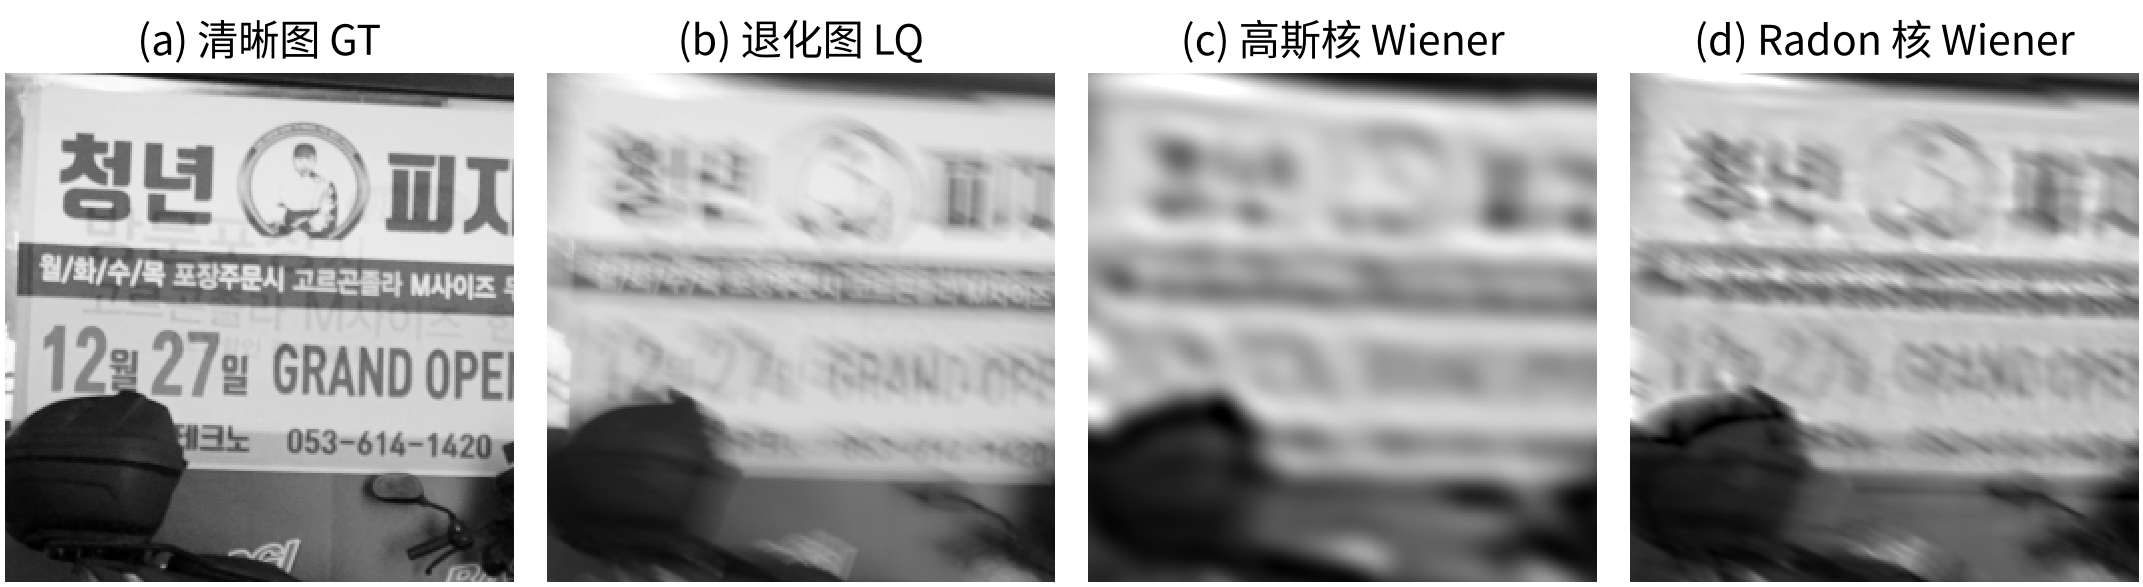
\includegraphics[width=\linewidth]{realblur_radon_crop.png}
\caption{RealBlur-J 选做对照。高斯猜核与 Radon 运动核采用相同 Wiener 参数 \(K=0.10\)}
\label{fig:radon}
\end{figure}
\FloatBarrier

\Needspace{8\baselineskip}
\section{结论}
在当前 DIV2K 合成样本上，已知 PSF 配合适当正则化能够改善轮廓与两项客观指标。
复原使用的循环卷积与周期退化边界一致时，外侧误差小于零填充及反射退化组。
RealBlur-J 的高斯猜核在主实验设置下不足以描述方向性模糊，Wiener 与 CLS 的画面出现明显振铃。
插值和 NLM 的指标只小幅变化，拖尾仍然存在。Radon 估计提供了更接近运动形式的全局近似，
但结果仍依赖正则化参数，且未恢复全部细节。
两组各使用一个场景，结论限定为对当前数据、模型与参数的比较。

\section{程序与复现}
实验使用 Python，核心依赖为 NumPy、OpenCV、SciPy、Matplotlib、scikit-image 和 pandas。
先运行任务一预处理，再运行任务二三个入口和任务三对照。
任务四直接调用任务二与任务三实现，统一生成图和评价表。下列命令依次复现必做部分，完整实现见附录。
\begin{Verbatim}[fontsize=\small]
MPLBACKEND=Agg python3 task1/task1.py
MPLBACKEND=Agg python3 task2/algorithm/code.py
MPLBACKEND=Agg python3 task2/param/param.py
MPLBACKEND=Agg python3 task2/realblur/realblur.py
python3 task3/task3.py
python3 task4/task4.py
\end{Verbatim}
选做核估计和比较入口位于 \texttt{task3\_extra}。依次执行
\path{radon_motion.py}、\path{wiener_k_test.py} 和 \path{compare_gaussian_radon.py}，
可以复现核估计、参数扫描与同参数对照。已有 RealBlur-J 运动核时，任务四会将选做结果加入汇总。
完整指标与边界诊断分别保存在
\path{task4/task4_metrics_summary.csv} 和 \path{task4/task4_artifacts_diagnostics.csv}。

\begingroup
\zihao{-5}
\bibliographystyle{gbt7714-numerical}
\bibliography{ref}
\endgroup

\clearpage
\appendix
\section*{附录\quad 实验代码}
\fvset{fontsize=\fontsize{8}{10}\linespread{1}\selectfont,
  formatcom=\CJKfamily{reportcode},numbers=left,numbersep=6pt,
  xleftmargin=2em,tabsize=4,breaklines=true,breakanywhere=true,
  breakautoindent=true,breakindent=1em,breaksymbolleft={},breaksymbolright={}}
\begingroup
\fvset{
  numbers=left,
  numbersep=0.6em,
  xleftmargin=2em,
  breaklines=true,
  breakanywhere=true
}

\section{图像预处理}
\subsection{\texttt{\detokenize{task1/task1.py}}}
\VerbatimInput{../../task1/task1.py}

\Needspace{90pt}
\section{传统频域图像复原}
\subsection{\texttt{\detokenize{task2/algorithm/code.py}}}
\VerbatimInput{../../task2/algorithm/code.py}

\Needspace{65pt}
\subsection{\texttt{\detokenize{task2/param/param.py}}}
\VerbatimInput{../../task2/param/param.py}

\Needspace{65pt}
\subsection{\texttt{\detokenize{task2/realblur/realblur.py}}}
\VerbatimInput{../../task2/realblur/realblur.py}

\Needspace{90pt}
\section{双三次插值与 NLM 对照}
\subsection{\texttt{\detokenize{task3/task3.py}}}
\VerbatimInput{../../task3/task3.py}

\Needspace{90pt}
\section{图像对比与指标评价}
\subsection{\texttt{\detokenize{task4/task4.py}}}
\VerbatimInput{../../task4/task4.py}

\endgroup


\end{document}
